An important fact is the property to suppress noise. In this section I will try to add some white Gaussian noise to the FM signal, generated by Matlab. The tolerated Signal-to-Noise-Ratio is specified to 40 dB. Below are some examples with different added noise.


\begin{figure}  
\begin{minipage}[t]{4.5cm}  
\begin{center}  
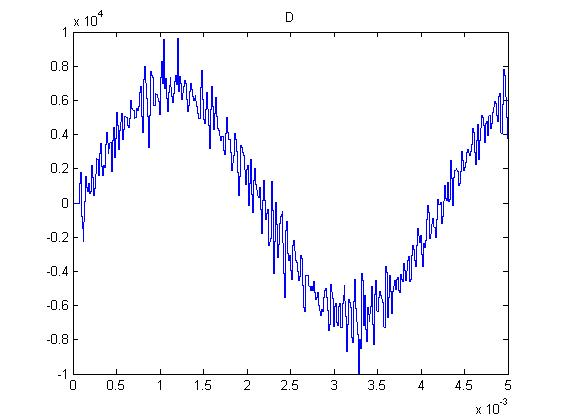
\includegraphics[width=8.0cm,clip]{images/13dBy.jpg}  
\caption[]{\label{fig:pure} Add white Gaussian noise to the input signal which is SNR = 40 dB, it yields 13,6 dB in SNR on output}  
\end{center}  
\end{minipage}  
\hfill  
\begin{minipage}[t]{7.5cm}  
\begin{center}  
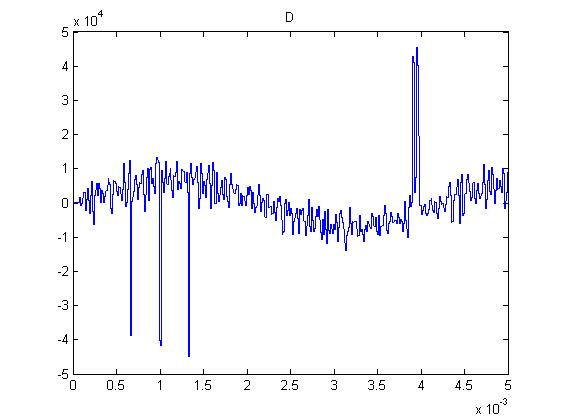
\includegraphics[width=8.0cm,clip]{images/noise4.jpg}  
\caption[Short caption for figure 2]{\label{fig:pure2} Add white Gaussian noise to the input signal which is SNR = 30 dB, it yields 4 dB in SNR on output}  
\end{center}  
\end{minipage}  
\end{figure}



\begin{figure}[h]
 \centering
 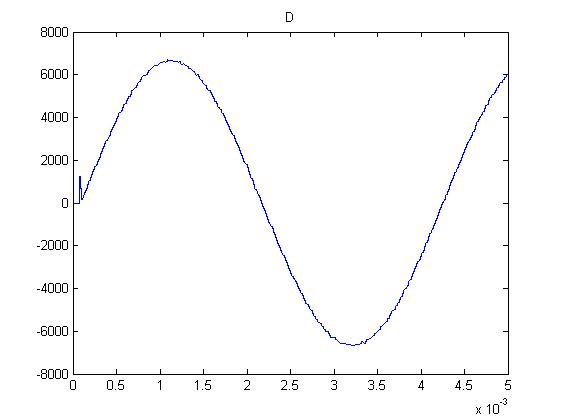
\includegraphics[scale=0.35]{images/noise40.jpg}
 \caption{Add white Gaussian noise to the input signal correspond to SNR = 70 dB, it yields 40 dB in SNR at output }
 \label{fig:pure3}
\end{figure}


It shows that the design not suppress the noise very well. It can be seen in figure \ref{fig:pure2} that a signal with SNR = 30 dB will enforce clicks back to the output again. The output will first be satisfied with a signal with SNR higher than 70 dB.
